\documentclass[tikz,border=4pt]{standalone}
\usepackage{amsmath}
\usetikzlibrary{calc,decorations.markings}
\begin{document}
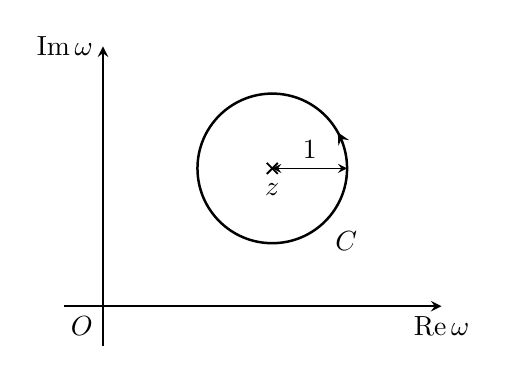
\begin{tikzpicture}[>=stealth, thick, scale=1.0]
  % Axes for complex omega-plane
  \draw[->, line width=0.7pt] (-0.5, 0) -- (4.3, 0) node[below] {$\mathrm{Re}\,\omega$};
  \draw[->, line width=0.7pt] (0, -0.5) -- (0, 3.3) node[left] {$\mathrm{Im}\,\omega$};
  \node[below left] at (0, 0) {$O$};

  % Center z and radius 1 circle C (counterclockwise)
  \coordinate (Z) at (2.15, 1.75);
  \draw[line width=0.9pt,
    postaction={decorate},
    decoration={markings, mark=at position 0.08 with {\arrow{>}}}
  ] (Z) circle (0.95);

  % Cross mark at z
  \draw[line width=0.7pt] ($(Z)+(-0.07,-0.07)$) -- ($(Z)+(0.07,0.07)$);
  \draw[line width=0.7pt] ($(Z)+(-0.07,0.07)$) -- ($(Z)+(0.07,-0.07)$);
  \node[below] at ($(Z)+(0,-0.06)$) {$z$};

  % Radius 1 arrow
  \draw[<->, line width=0.45pt] (Z) -- ++(0.95, 0) node[midway, above] {$1$};

  % Contour label C
  \node[below right] at ($(Z)+(-45:0.95)$) {$C$};
\end{tikzpicture}
\end{document}
